\section{Solid particles at fluid interfaces}

This strong attachment energy makes particles highly effective at stabilizing emulsions by becoming irreversibly trapped at fluid-fluid interfaces. 
\cite{ngai_particle-stabilized_2015}Once adsorbed, these 
particles reduce interfacial tension and act as physical barriers that prevent the coalescence of droplets, thereby enhancing emulsion stability. Unlike molecular surfactants, 
which are dynamic and can desorb under certain conditions, colloidal particles remain anchored at the interface due to the significant energy required to detach them. 
\cite{ngai_particle-stabilized_2015}This mechanism 
is especially useful in systems such as Pickering emulsions, where the interfacial coverage and wettability of the particles determine the type and stability of the emulsion formed. 
\cite{ngai_particle-stabilized_2015,velankar_non-equilibrium_2015}
As such, understanding particle behavior at interfaces is essential for controlling the structure and longevity of particle-stabilized systems. \cite{ngai_particle-stabilized_2015}
For particles that are smooth and simple and at an interface of oil and water, the attachment energy at the fluid interface can be calculated from a force 
balance between the force imparted from the particle on each fluid and the fluids between one another, known as the Young-Dupre equation.

\begin{equation}
    \cos{\theta_c} = \frac{\sigma_{po} - \sigma_{pw}}{\sigma_{ow}}
\end{equation}

Where $\theta_c$ is the contact angle, $\sigma_{po}$ is the surface tension between particle and oil, $\sigma_{pw}$ is the surface tension between particle and water and
$\sigma_{ow}$ is the surface tension between oil and water. The particle is considered to be preferentially wet by water or hydrophilic if $\theta_c < 90 ^{\circ}$ or 
hydrophobic if $\theta_c > 90 ^{\circ}$. The particle is said to be neutrally wetting if $\theta_c = 90 ^{\circ}$. 

\begin{figure}
    \centering
    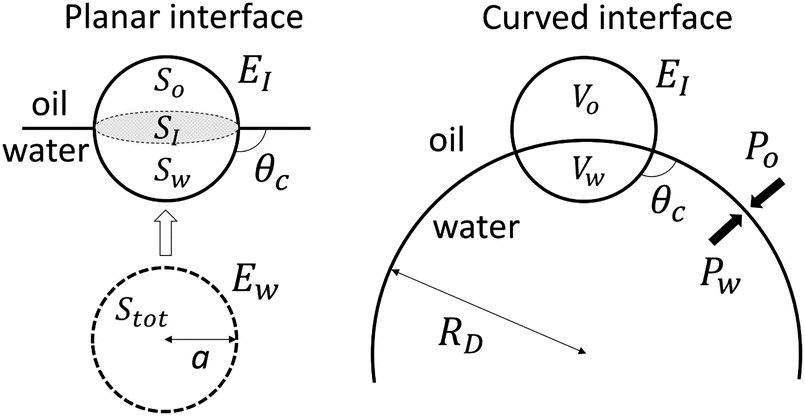
\includegraphics[scale = 0.5]{../figures/literature_review/particle_at_interface.png }
    \caption{Particle schematic at an interface demonstrating the various quantities of interest. Reprinted Figure 2.1 with permission from
             Particle-Stabilized Emulsions and Colloids: Formation and Applications; Ngai, T., Bon, S. A. F., Eds.; RSC soft matter series; 
             Royal Society of Chemistry, RSC Publishing Cambridge, 2015}
    \label{fig:pieranski_model}
\end{figure}

The energy of the system before and after particle adsorption is different and can be characterized for a simple system with parameters shown in Figure \ref{fig:pieranski_model},

\begin{equation}
    \Delta E_{IW} = E_I - E_w
\end{equation}

Where $\Delta E_{I}$ is the energy of the system when the particle is in the interface and $\Delta E_W$ is the energy of the system when the particle is completely in the water phase.
We define $\Delta E_{I}$ as

\begin{equation}
    E_I = A_w \sigma_{pw} + A_o\sigma_{po} + A_{I_1}\sigma_{ow} + V_w P_w + V_o P_o
\end{equation}

Where $A_w$ and $A_o$ are the surface areas of the particle in the water and oil phases respectively, $V_w$ and $V_o$ are the volumes of water and oil phases respectively and 
$P_w$ and $P_o$ are the pressures of water and oil phases respectively. $A_{I_1}$ is the area of the interface with the particle. 
A similar equation can be written for the energy of the water phase, $E_w$

\begin{equation}
    E_w = (A_w + A_o)\sigma_{pw} + A_{I_2}\sigma_{ow} + (V_w + V_o)P_w
\end{equation}

$A_{I_2}$ is the area of the interface without the particle. The change in the interface energy upon adsorption of the particle can be computed to obtain

\begin{equation}
    \Delta E_{IW} = A_o(\sigma_{po} - \sigma_{pw}) - A_p\sigma_{ow} + V_o(P_o - P_w)
\end{equation}

Substituting the Young-Laplace law for a spherical droplet, $P_w - P_o = \frac{2\sigma_{ow}}{R_d}$ where $R_d$ is the droplet size, for $(P_o - P_w)$ and the Young-Dupre contact angle
expression, the following is obtained

\begin{equation}
    \Delta E_{IW} = \sigma_{ow}(A_o\cos{\theta_c} - A_p - \frac{2 V_o}{R_d})
\end{equation}

A similar construction can be done for the oil phase to obtain 

\begin{equation}
    \Delta E_{IW} = -\sigma_{ow}(A_w\cos{\theta_c} + A_p - \frac{2 V_o}{R_d})
\end{equation}

After making appropriate geometrical substitutions for $V_o$ and $A_p$, the Piersanski model is recovered,

\begin{equation}
    \Delta E_{ads} = \pi r^2 \sigma_{ow} (1 - |\cos{\theta_c}|)^2
\end{equation}

From this expression, the adsorption energy can be seen to depend on the contact angle, surface tension and contact area of the particles. This indicates that larger, neutrally wetting
particles adsorbing onto interfaces with high surface tension have a high driving force for adsorption. \cite{ngai_particle-stabilized_2015,reeves_particle-size_2015} This adsorption process 
can be orders of magnitude larger than the thermal energy of the system, calculated as $k_b T$ where $T$ is the temperature of the system and $k_b$ is the Boltzmann constant. This results in 
irreversible adsorption of particles at interfaces. \cite{binks_pickering_2001}

In addition to the adsorption of particles on the interface, the contact angle of the particles determine the dispersed phase of an emulsion and its microstructure. 
\cite{velankar_non-equilibrium_2015}
Hydrophillic particles tend to prefer to form oil in water emulsions while hydrophobic particles prefer to form water in oil emulsions. \cite{ngai_particle-stabilized_2015}
This occurs as the particles preferentially wet one phase over another, causing the interface to bend as the emulsion forms. Neutrally wetting particles are preferred in the formation of 
bijels as no preferential curvature is imparted onto the bijels, fulfilling one of the requirements of a minimal surface in that the mean curvature must be zero. \cite{jinnai_interfacial_2001}

\section{Phase separation}

To understand the formation of bijels, the difference between nucleation and growth and spinodal decomposition must be understood. These processes 
govern how distinct domains emerge and evolve within a binary mixture upon quenching into the two-phase region of the phase diagram. While nucleation and growth involve the formation 
and expansion of isolated domains, spinodal decomposition leads to the spontaneous, interconnected structuring characteristic of bijels. Investigating both mechanisms provides insight 
into how thermodynamic and kinetic pathways influence the resulting microstructure, and why spinodal decomposition is uniquely suited for producing the bicontinuous 
architecture essential to bijels. A schematic free energy and phase diagram is plotted in Figure \ref{fig:phase_diagram}

\begin{figure}
    \centering
    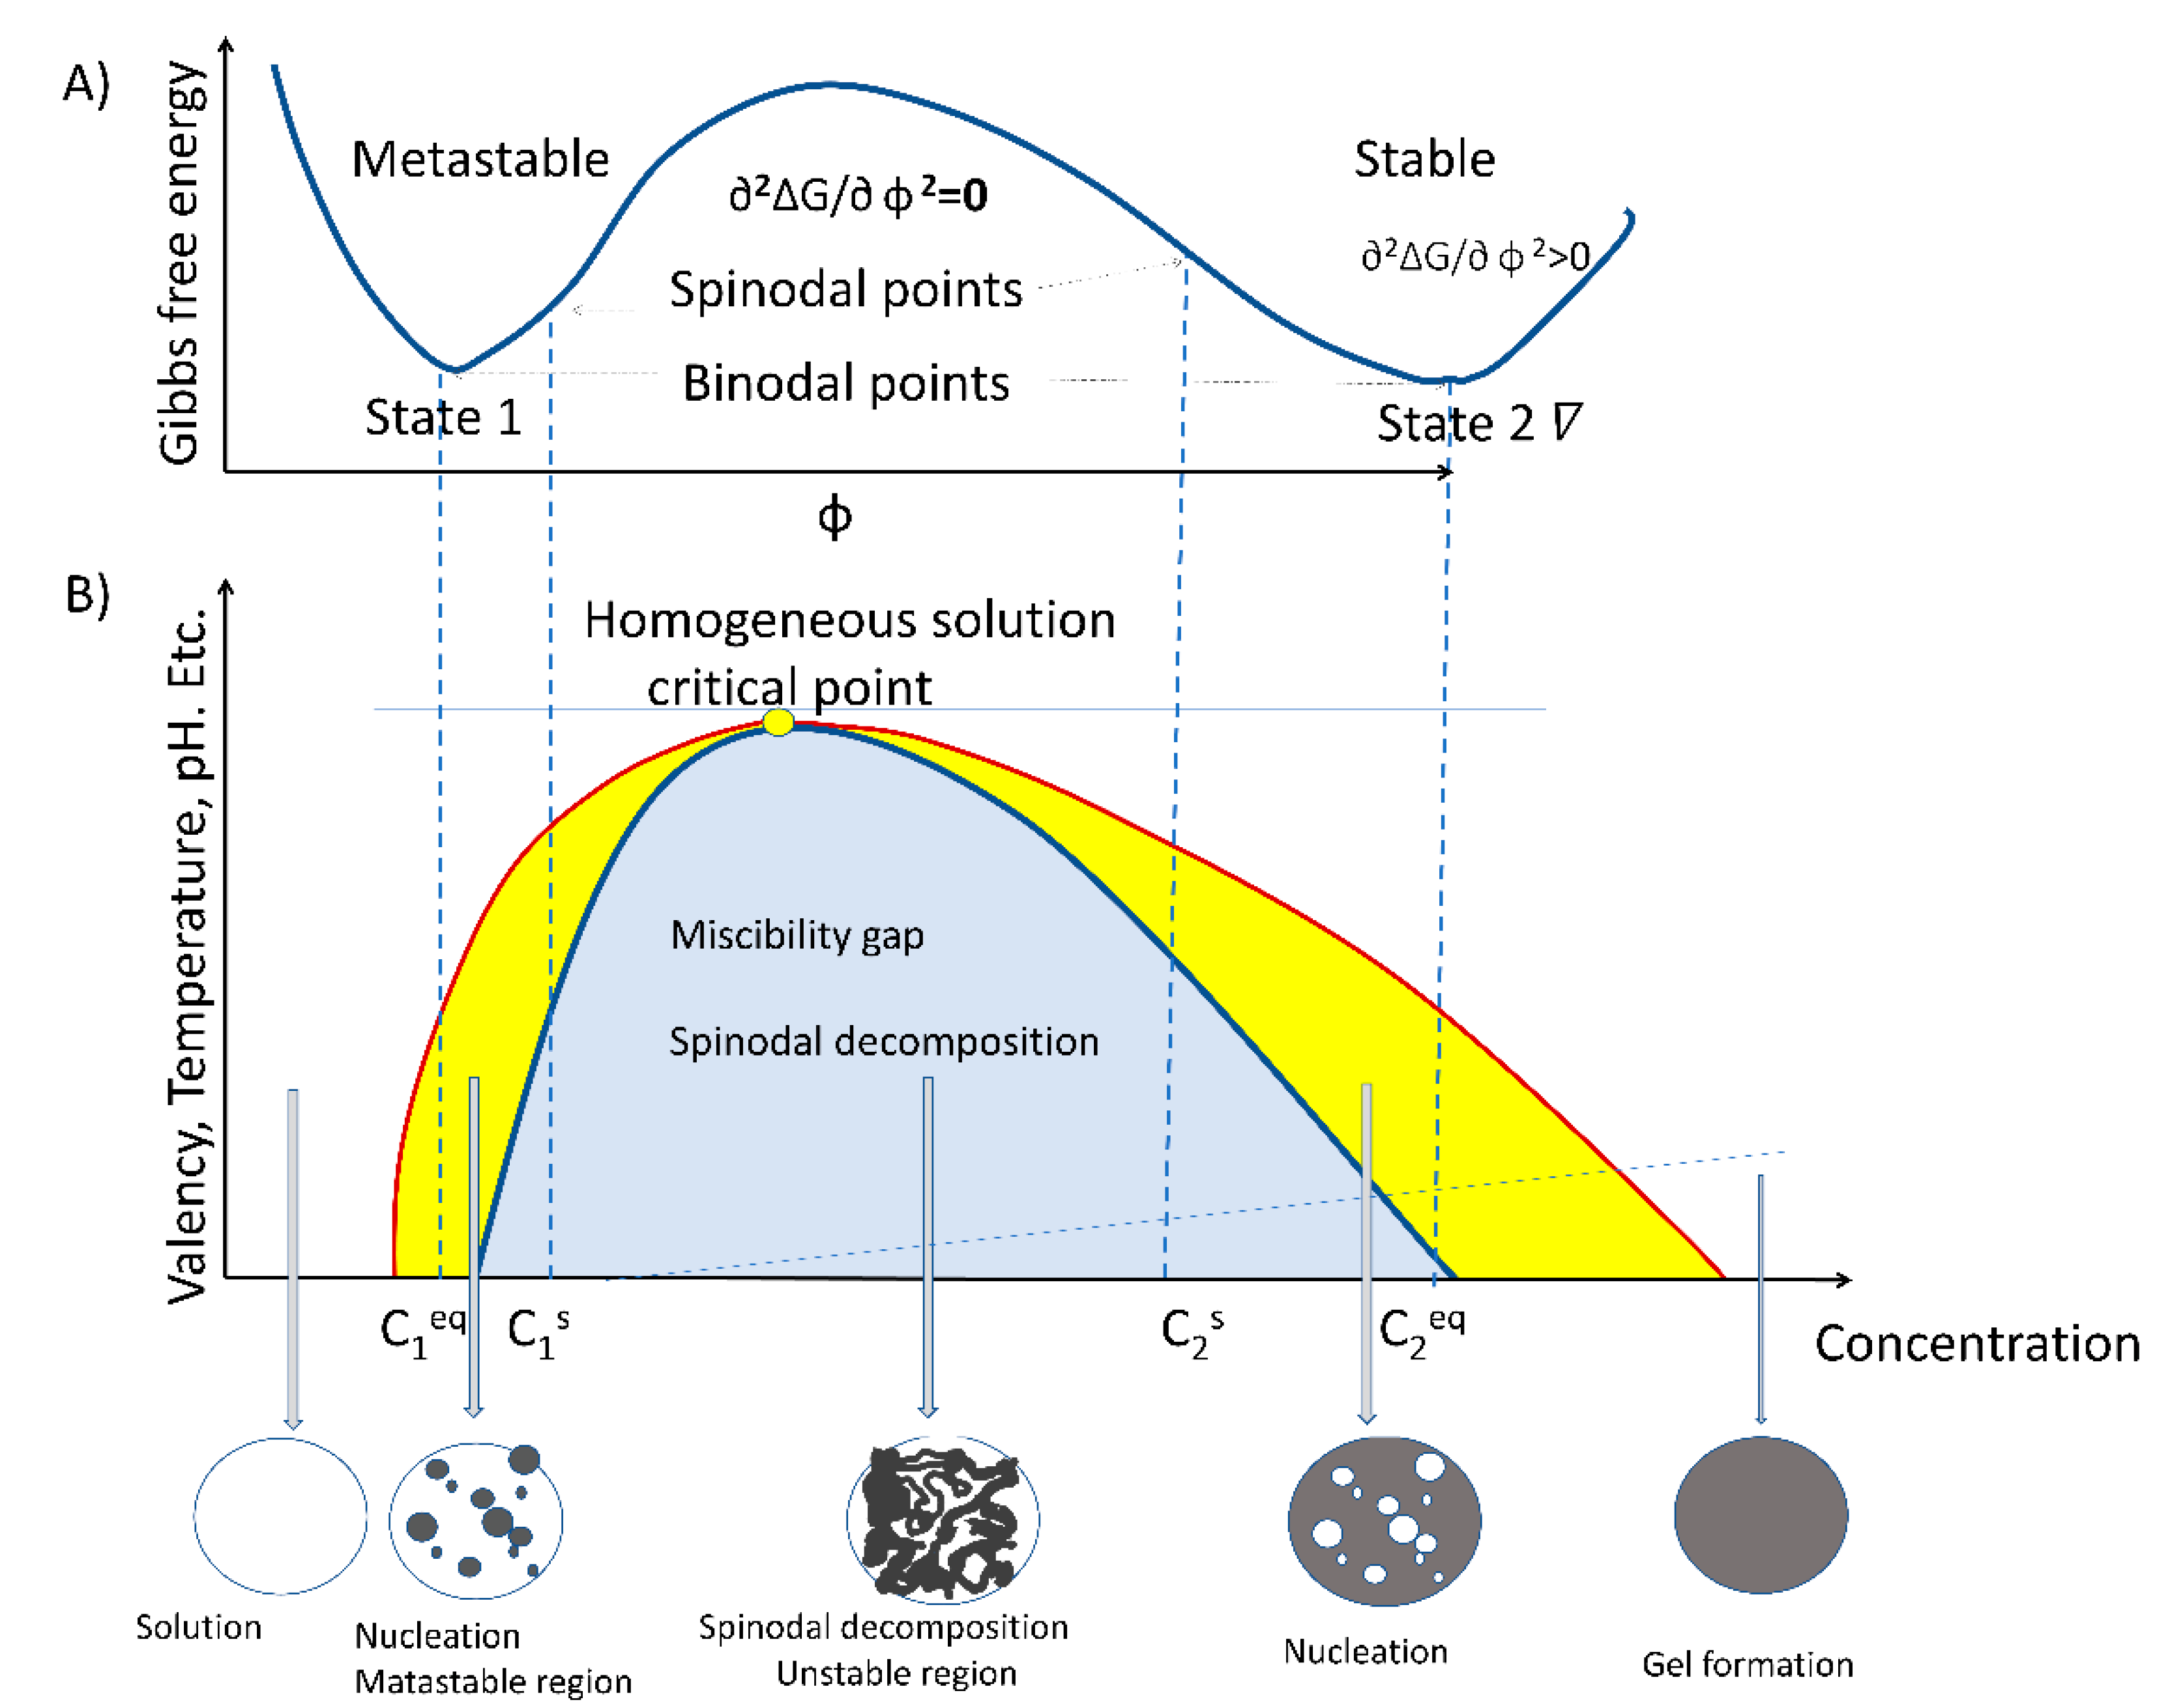
\includegraphics[scale = 0.7]{../figures/literature_review/phase_diagram.png}
    \caption{Schematic of a phase diagram obtained from a free energy curve demonstrating key features of the free energy landscape that correspond
             to the phase diagram. Reprinted Figure 1 from
             Guillen-Chable, F.; Bayona, A.; Rodríguez-Zapata, L. C.; Castano, E. Phase Separation of Intrinsically Disordered 
             Nucleolar Proteins Relate to Localization and Function. IJMS 2021, 22 (23), 13095. with permission under the Creative Common CC BY license.}
    \label{fig:phase_diagram}
\end{figure}

The thermodynamic equilibrium of a binary fluid mixture can be described by its Gibbs free energy, given as \(\Delta G = \Delta H - T \Delta S\), where \(\Delta H\) is the enthalpy change, 
\(T\) is temperature, and \(\Delta S\) is the entropy change. The onset of phase separation occurs at the binodal line, defined where \(\frac{dG}{dx} = 0\), with \(x\) representing the composition. 
Although the system is metastable, it remains uniform until fluctuations give rise to small nuclei. The free energy of each nucleus reflects a 
balance between the bulk free energy gain from phase separation and the interfacial energy penalty, expressed as \(\Delta G = \frac{4}{3}\pi r^3 \Delta g_v + 4 \pi r^2 \sigma\), where \(r\) is 
the nucleus radius, \(\Delta g_v\) is the free energy change per unit volume, and \(\sigma\) is the interfacial tension. 
\cite{thanh_mechanisms_2014}
Nuclei that exceed the critical radius \(r_c = \frac{2\sigma}{|\Delta g_v|}\) will grow, driving the system toward phase separation via nucleation and growth. \cite{thanh_mechanisms_2014}
This transformation process is commonly modeled by the Avrami equation, \(Y = 1 - \exp(-K t^n)\), where \(Y\) is the 
transformed fraction, \(K\) is a rate constant incorporating nucleation and growth kinetics, and \(n\) is the Avrami exponent, which reflects the dimensionality and mechanism of the transformation.
\cite{avrami_kinetics_1939}

At the binodal, the system is still metastable, meaning that unless perturbations are introduced to form nuclei, the mixture remains homogeneous. \cite{thanh_mechanisms_2014}
However, a deeper quench into the two-phase region leads to the spinodal line, defined by the stability criterion \(\frac{d^2G}{dx^2} = 0\). \cite{cahn_free_1958}
Within this region, the system is unstable to even infinitesimal composition fluctuations, and phase 
separation proceeds spontaneously without the need for nucleation. This process, known as spinodal decomposition, is characterized by the continuous and simultaneous growth of interconnected 
domains of both phases. \cite{cahn_free_1958} Unlike nucleation and growth, which relies on localized events, spinodal decomposition 
results in a bicontinuous structure driven by the system's attempt to minimize 
free energy through composition modulation. \cite{cahn_free_1958} The dynamics of spinodal decomposition were characterized by Cahn and Hilliard. \cite{cahn_free_1958} 
We first begin by defining the free energy of a regular solution, known as the bulk free energy.

\begin{equation}
    \Delta G_m = \chi (1 - \phi)\phi + N_a k_B T \left[(1 - \phi)\ln(1 - \phi) + \phi \ln(\phi)\right]
\end{equation}

This bulk free energy characterizes the thermodynamic driving forces for phase separation. Alternative forms, such as the Landau-Ginzburg or Flory-Huggins models, may also be used depending on system 
specifics. In real systems, the interface between two partially miscible fluids is not sharp, meaning that the composition transitions smoothly across a finite interface width. To account for this, a 
gradient energy penalty is added to the free energy functional, penalizing sharp spatial variations in composition. The total free energy functional is written as

\begin{equation}
    F[\phi] = \int \left( f(\phi) + \frac{\kappa}{2}|\nabla \phi|^2 \right) \, dV
\end{equation}

where $\kappa$ is the gradient energy coefficient controlling the interface width. Larger \(\kappa\) values correspond to wider interfaces.
The chemical potential is then defined as the variational derivative of the free energy functional,

\begin{equation}
    \mu = \frac{\delta F}{\delta \phi} = \frac{df}{d\phi} - \kappa \nabla^2 \phi
\end{equation}

This chemical potential enters the mass flux expression via a Fickian transport law,

\begin{equation}
    \vec{J} = -M \nabla \mu
\end{equation}

where $M$ is the mobility and could potentially be a function of $\phi$. Assuming no advection and applying mass conservation for the order parameter, we obtain,

\begin{equation}
    \frac{\partial \phi}{\partial t} = -\nabla \cdot \vec{J}
\end{equation}

Substituting in the expression for \(\vec{J}\) leads to the Cahn-Hilliard equation \cite{cahn_free_1958},

\begin{equation}
    \frac{\partial \phi}{\partial t} = \nabla \cdot \left( M \nabla \mu \right)
\end{equation}

This equation describes the diffusive evolution of the conserved field $\phi$ during phase separation. It captures the system's tendency to minimize its total free energy 
by redistributing the order parameter according to gradients in chemical potential. The Cahn-Hilliard framework naturally incorporates interfacial tension and allows for smooth, 
continuous transitions between phases, making it highly suitable for modeling non-ideal mixing in systems such as bijels.

The most important difference between these two phase separation methods is the morphology of the phase separated structure. While nucleation and growth generates discontinuous droplets,
spinodal decomposition creates continuous domains that have tunable domain sizes and tortuosity which are attractive in many materials applications such as battery electrodes, filtration
membranes and catalyst supports.

\section{Anisotropic particles}

As the library of available particle shapes continues to grow, it becomes increasingly important to understand how these anisotropic particles behave at fluid interfaces.
\cite{wu_recent_2016, cavallaro_curvature-driven_2011}
Unlike spherical particles, anisotropic particles introduce directional interactions and complex rotational dynamics which can significantly 
influence interfacial assembly and emulsion stability. \cite{read_dimerization_2020, davies_dipolar_2015,morgan_understanding_2013}
Their shape can dictate not only their orientation at the interface but also how they interact, and jam, 
ultimately affecting the structure and mechanical properties of the resulting material. \cite{hijnen_bijels_2015}
This is relevant for systems like bijels, where the precise arrangement of particles at the interface affects how the bijel james in place, generating new timescales or 
interfacial phenomena not characterized in bijels made with spheres. \cite{gunther_timescales_2014,hijnen_bijels_2015} 

Anisotropic particles exhibit shape-dependent interfacial behavior due to their ability to induce complex multipolar capillary interactions. When adsorbed at a fluid-fluid interface, these 
particles distort the surrounding interface in order to maintain a mean curvature of zero, in accordance with the Young-Laplace equation. This distortion creates curvature gradients around the 
particle that interact with nearby particles or features on the interface, giving rise to anisotropic capillary forces. \cite{loudet_capillary_2005, cheng_shape-anisotropic_2013}. 
Computational simulations further support this complexity, showing that ellipsoidal particles can adopt a variety of metastable orientations 
depending on initial conditions and perturbations encountered during adsorption or rearrangement at the interface \cite{gunther_lattice_2013, newton_influence_2014}. 

\begin{figure}
    \centering
    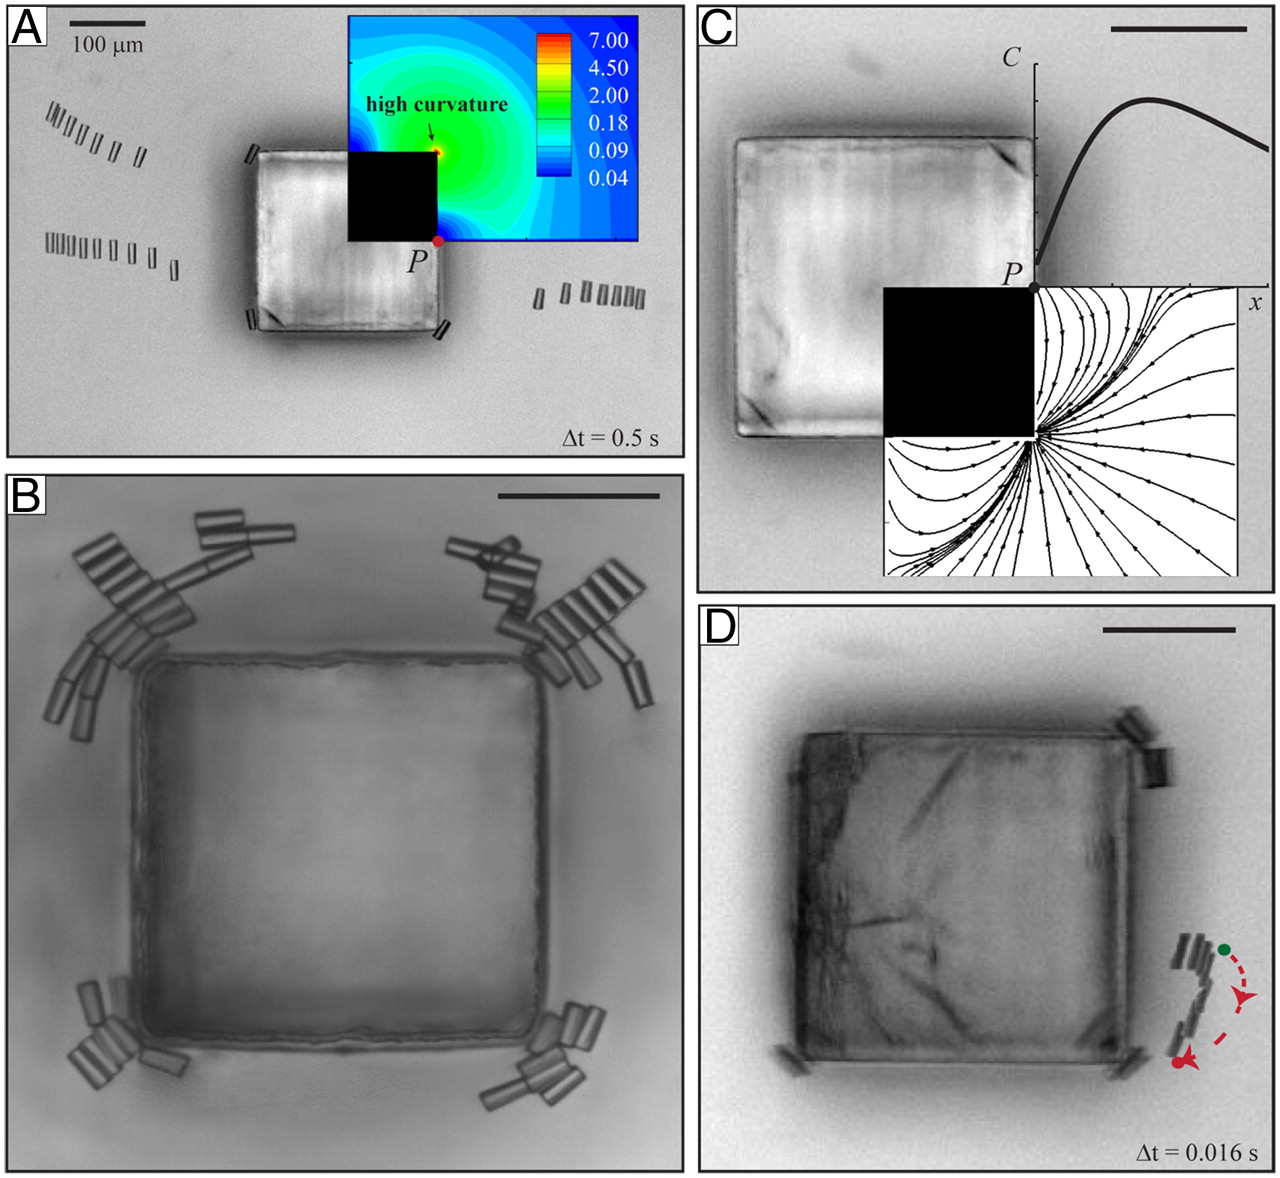
\includegraphics[scale = 0.3]{../figures/literature_review/curvature_driven_assembly.jpeg}
    \caption{Self assembly of particles at points of large curvature gradients. Reproduced from Figure 5 in Cavallaro, M.; Botto, L.; 
             Lewandowski, E. P.; Wang, M.; Stebe, K. J. Curvature-Driven Capillary Migration and Assembly of Rod-like Particles. 
             Proc. Natl. Acad. Sci. U.S.A. 2011, 108 (52), 20923-20928 under the CC-BY license}
    \label{fig:curvature_gradient}
\end{figure}

When looking at arrays of ellipsoidal particles at interfaces, curvature gradients control the dynamics of the system. Figure \ref{fig:curvature_gradient} illustrates the effect that
Cavallaro and co-workers identified. They showed how curvature gradients created at the edges of a 
square rod caused directed assembly of cylinders, with the driving force strong enough to overcome gravity. \cite{cavallaro_curvature-driven_2011} Other works have introduced how these features are 
particle shape dependent with greater control over the curvature gradient providing a means to control particle self assembly. \cite{read_dimerization_2020, sharifi-mood_curvature_2015} Botto et al. 
identified that ellipsoidal particles prefer to arrange side to side state while cylinders prefer to arrange tip to tip with the particle geometric smoothness playing a role in this preference.
\cite{botto_capillary_2012} These differences in particle arrangement could open up new possibilities for tailoring interfacial assemblies and the subsequent differences in microstructure obtained in
a bijel.

Ellipsoidal particles have been used as stabilizers in bijels, resulting in bijels that have smaller domains than those made with spherical particles at the same volume fraction. This was identified to arise 
from the greater surface area to volume ratio of ellipsoidal particles compared to spherical particles. \cite{gunther_timescales_2014} The evolution of the microstructure is also distinct to bijels 
stabilized with spheres, demonstrating two timescales at early and later timesteps. \cite{gunther_timescales_2014} The short timescale is during formation of the bijel, when particles are adsorbed onto the
interface and rotate to align with the interface. At longer timescales, capillary interactions between particles lead to reordering of particles at the interface, leading to a different interfacial 
configuration and microstructure. \cite{gunther_timescales_2014}

\begin{figure}
    \centering
    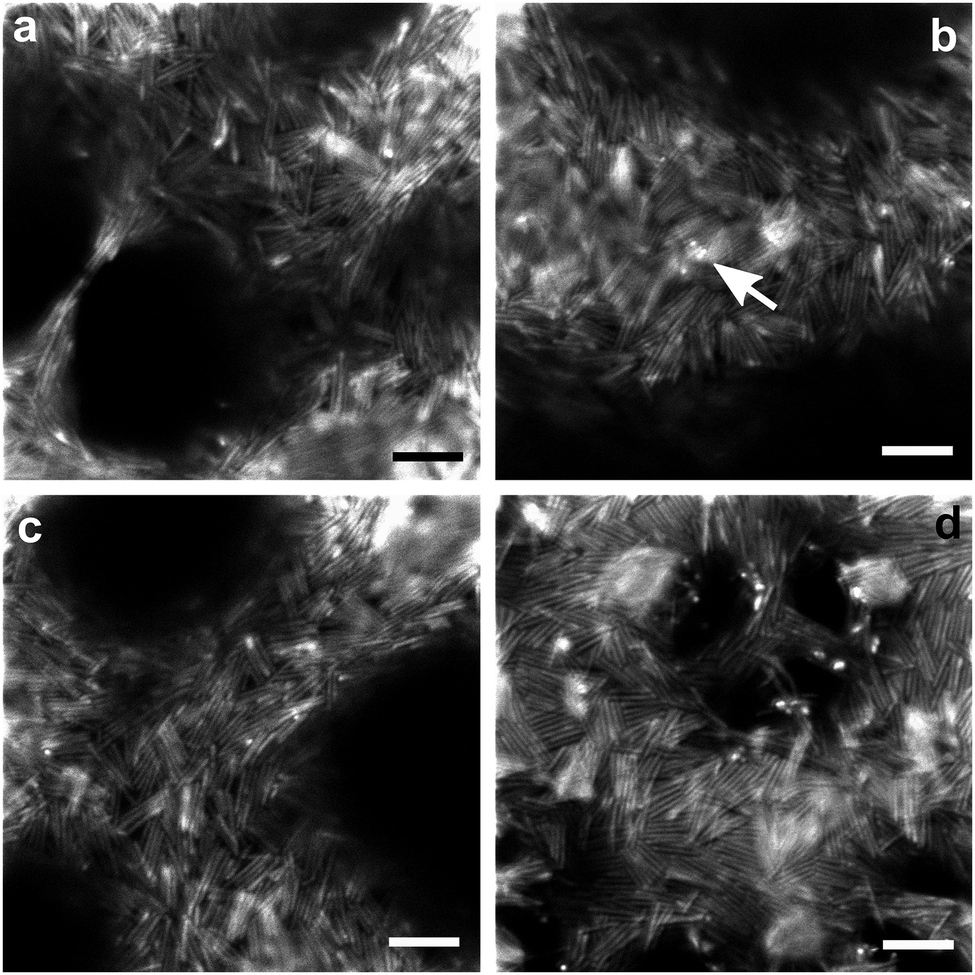
\includegraphics[scale = 0.3]{../figures/literature_review/rods_bijels.png}
    \caption{Bijels stabilized by rod like particles, demonstrating 'flippers' at the interface, which are particles that flip out of the interface due to stress from adjacent particles. 
             Reproduced from Figure 3 in Hijnen, N.; Cai, D.; Clegg, P. S. Bijels Stabilized Using Rod-like Particles. Soft Matter 2015, 11 (22), 4351-4355 under the CC-BY license}
    \label{fig:rod_bijel_flippers}
\end{figure}


Rod like particles have also been used as stabilizers in experiments, identifying that the length scale of the pores of the bijels follows $ L \propto \frac{1}{\phi_p} $ even if the proportionality constant 
is different. Figure \ref{fig:rod_bijel_flippers} demonstrates bijels stabilized by rod like particles showing that particles flip out of the interface due to steric forces from adjacent particles. This
flipping can increase the resistance to shear due to capillary bridging between adjacent rods.
While the proportionality constant depends on particle geometry, this trend has been observed across various particle shapes 
\cite{hijnen_bijels_2015, madivala_exploiting_2009, gunther_timescales_2014, daware_emulsions_2015, loudet_capillary_2005, cheng_shape-anisotropic_2013}. 
The dynamics of bijels stabilized by ellipsoidal particles are also distinct from bijels stabilized by spheres, caused by reorientation of particle stabilizers at the interface. \cite{gunther_timescales_2014}

\section{Rheology}

Understanding the rheology of emulsions, particularly bijels, is essential because it directly impacts both their fabrication and practical use. \cite{haase_situ_2016}
Previous investigations have characterized that bijels are non-Newtonian fluids with a yield stress and shear thinning behavior. \cite{macmillan_rheological_2019}
A non-Newtonian fluid is one whose viscosity is not constant but varies with the applied shear rate or stress. In Newtonian fluids like water 
or air, there is a linear relationship between shear stress and shear rate, meaning viscosity remains the same regardless of how fast the fluid is sheared. \cite{mezger_rheology_2020} Non-Newtonian fluids, on 
the other hand, deviate from this behavior and may exhibit shear thinning, shear thickening, yield behavior or viscoelasticity with no fluid constrained to one behavior. \cite{mezger_rheology_2020}
Shear thinning and thickening here define that the change in viscosity is sub-linear and super-linear respectively, while yield behavior implies that the viscosity is non-zero when no shear 
is applied. \cite{mezger_rheology_2020} Viscoelasticity appears when the shear response of the fluid is dependent upon the frequency of the applied shear, indicating that the fluid has both liquid and solid like 
characteristics. \cite{mezger_rheology_2020}
These properties often appear in soft matter and multiphase systems where microstructure and particle interactions influence flow behavior.

\begin{figure}
    \centering
    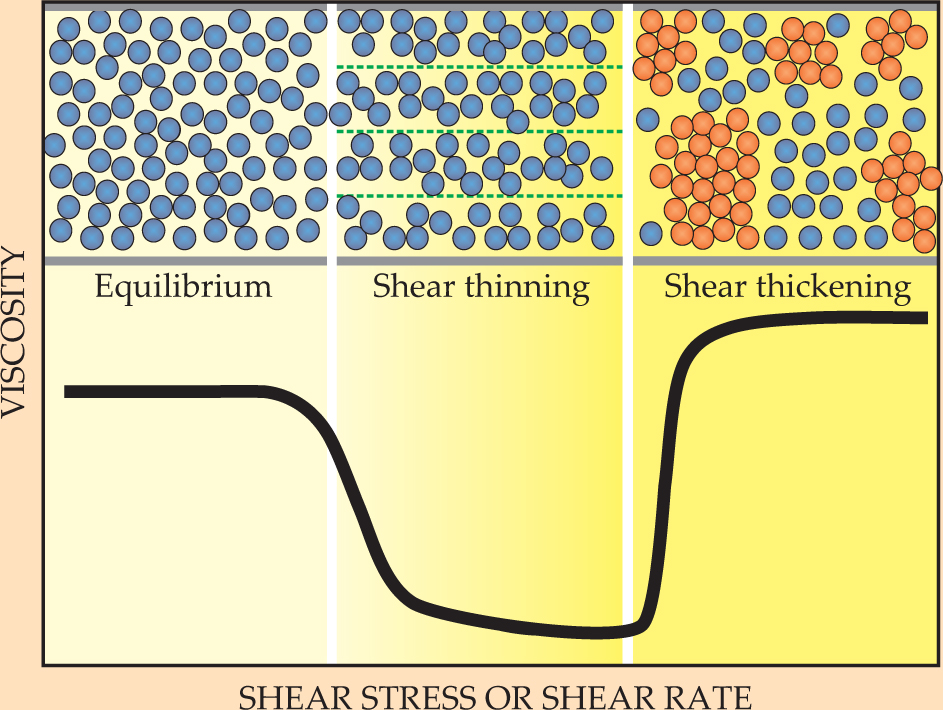
\includegraphics[scale = 0.3]{../figures/literature_review/shear_suspensions.jpeg}
    \caption{Schematic of suspensions under shear demonstrating shear banding and shear aggregates modifying the rheological properties of a suspension. 
             Reproduced from Figure 2 in Wagner, N. J.; Brady, J. F. Shear Thickening in Colloidal Dispersions. Physics Today 2009, 62 (10), 27-32 under the CC-BY license}
    \label{fig:suspension_shear}
\end{figure}

Suspensions and emulsions are examples of non-Newtonian fluids due to the presence of dispersed particles or droplets within a continuous phase. 
\cite{brader_nonlinear_2010, besseling_three-dimensional_2007, xu_relation_2013}  
In suspensions, the interaction  between solid particles—such as hydrodynamic forces, electrostatic repulsion, and steric hindrance—creates microstructural rearrangements under flow, leading to 
non-linear viscosity 
responses. \cite{brader_nonlinear_2010, besseling_three-dimensional_2007} Figure \ref{fig:suspension_shear} demonstrates the shear properties of an example suspension, demonstrating how shear thinning
and shear thickening can occur in suspensions. At low shear, particles may aggregate or form a network that resists deformation, while higher shear rates can break 
down these structures, resulting in shear thinning. In dense systems, particles may experience contact-induced resistance or jamming, causing shear thickening. \cite{brader_nonlinear_2010}

Emulsions behave similarly with droplet deformation, coalescence, and interactions 
among droplets generating time-dependent and non-linear responses to shear. When particles are used to stabilize emulsions (e.g., in Pickering emulsions), their interfacial rigidity 
adds further resistance to flow and deformation, contributing to complex, often viscoelastic, rheological behavior.
Madivala et al. showed that Pickering emulsions stabilized with rod-like particles had enhanced stability under shear, with greater resistance observed as particle aspect ratio increased 
\cite{madivala_exploiting_2009}. They identified this improvement to be due to improved interfacial coverage of ellipsoidal particles at interfaces and the improved elasticity of the interface,
allowing for the droplet to elongate more before failure. These improvements also extend to disc like particles with other investigations into the resistance to shear of emulsions stabilized by
graphene nanosheets, showing that they were able to provide better resistance to shear than spherical particles. \cite{imperiali_simple_2014} This was due to the graphene nanosheets overlapping one
another during shear, creating greater resistance to the applied shear and a higher apparent viscosity. In this case too, the overlap of graphene nanosheets was shown to result in greater interfacial
elasticity inferred through surface tension measurements of droplets with graphene stabilizers. \cite{sun_assembly_2013}

\begin{figure}
    \centering
    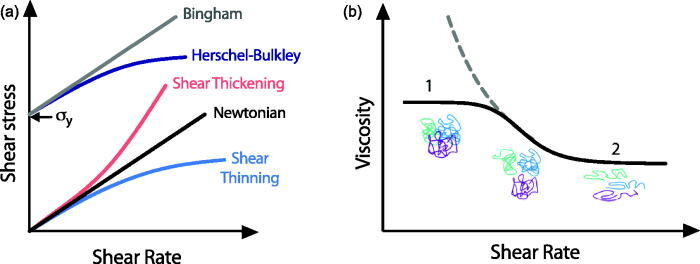
\includegraphics[scale = 4]{../figures/literature_review/Flow-curves.png}
    \caption{Schematic of expected shear stress as a function of applied shear rate for various models of fluids on the left and a shear thinning material on the right, demonstrating
             the yield stress at low strain rate followed by shear thinning and the infinite shear rate plateau. Reproduced from Cooke, M. E.; Rosenzweig, D. H. The Rheology of Direct 
             and Suspended Extrusion Bioprinting. APL Bioengineering 2021, 5 (1), 011502 under the CC BY license.}
    \label{fig:shear_theory}
\end{figure}

Several theoretical models have been developed to describe the behavior of non-Newtonian fluids under constant shear. The schematic representation of these models is shown in
Figure \ref{fig:shear_theory}. The power law Model is commonly used to represent shear thinning or 
thickening, with the equation \(\sigma = k \dot{\gamma}^n\), where \(\sigma\) is shear stress, \(\dot{\gamma}\) is shear rate, \(k\) is the consistency index, and \(n\) is the flow index.
\cite{mezger_rheology_2020}
For \(n<1\), the fluid is shear thinning and for \(n>1\), shear thickening. \cite{mezger_rheology_2020}
The Bingham plastic model and Herschel-Bulkley model account for yield stress, with the latter being more general by 
including power-law behavior after yielding, defined as $\sigma = \sigma_y + k \dot{\gamma}^n$. \cite{mezger_rheology_2020}
Shear models that include viscoelasticity have also been developed such as the  Maxwell and Kelvin-Voigt 
models. \cite{mezger_rheology_2020}
They are used when the fluid exhibits both solid- and liquid-like characteristics under stress, incorporating time-dependent strain responses and relaxation phenomena. These models help 
predict and quantify the behavior of complex fluids in real-world applications. \cite{mezger_rheology_2020}

Bicontinuous interfacially jammed emulsion gels (bijels) exhibit highly complex rheological behavior due to their unique microstructure. Bijels typically show yield stress and viscoelasticity, 
behaving like soft solids under low stress and flowing under high stress. \cite{macmillan_rheological_2019, bai_dynamics_2015, lee_making_2013}  The rigidity of the 
particle-laden interface resists deformation, until the applied shear rate is high enough to overcome the frictional contacts keeping particles in place. \cite{boakye-ansah_controlling_2020} 
Experimental studies have reported non-Newtonian behavior such as shear thinning, attributed to the gradual inability of the particles to resist shear. \cite{macmillan_rheological_2019}
Simulation studies using Lattice Boltzman have identified the failure mechanism of bijels stabilized by spherical particles to be due to shear induced ordering to the applied field before
particle ejection from the interface, causing domain coalescence. \cite{bonaccorso_shear_2020} However, the rheology of bijels is still an emerging field, 
with ongoing work focused on understanding how particle properties such as shape, particle size and contact angle affect flow behavior. One important find was that bijels were 
2D colloidal glasses percolating in 3D. \cite{ching_bijel_2022}

Magnetic fields introduce a means of dynamically tuning the rheology of emulsions stabilized by magnetically responsive particles. 
\cite{qiao_magnetorheological_2012} In Pickering emulsions, magnetic fields can induce droplet deformation and change the rigidity of the particle monolayer, thereby changing the flow behavior. 
\cite{qiao_magnetorheological_2012} For bijels incorporating magnetic particles, external fields can affect the stability and 
elasticity of the interfacial particle layer or cause domain reorganization. These effects can lead to tunable yield stress, viscosity, and viscoelastic properties.

\section{Emulsion studies using Lattice Boltzmann}

Understanding the complex interplay between fluid phases and particles in emulsions requires modeling approaches that can capture hydrodynamic interactions, interfacial tension, and particle 
behavior at mesoscopic scales. The multicomponent Lattice Boltzmann method has emerged as a powerful tool for simulating such systems, as it bridges the gap between continuum fluid dynamics 
and molecular-level detail. LB models can naturally incorporate smooth interfaces, phase separation dynamics, and solid-fluid coupling, making them particularly well-suited for studying 
emulsion formation, coarsening, and stabilization mechanisms. This has enabled detailed investigations into how particle properties and flow conditions influence emulsion structure and rheology.

One significant contribution of LB simulations to emulsion research has been the study of dynamical scaling during spinodal decomposition, characterized as the growth of the lengthscale
over time following a power law behavior. \cite{siggia_late_1979, furukawa_role_1994} From the multicomponent Navier Stokes equation, Reynolds number dependent scaling exponents for the 
lengthscale of the system were identified that were termed the viscous limit, where the Reynolds number was low, and the inertial limit, where the Reynolds number is high. \cite{kendon_inertial_2001} 
Multicomponent LB studies definitively demonstrated the ranges of Reynolds number where these scaling laws held and identified a broad crossover region. \cite{kendon_inertial_2001, kendon_3d_1999}

Additionally, the bijel itself was first realized computationally using LB simulations. \cite{stratford_colloidal_2005} A multicomponent LB model with neutrally wetting colloids based on the implementation
by Ladd showed that coarsening interfaces could catch particles irreversibly adsorbing them and arresting coarsening once the interfacial area matched the cross sectional area of particles adsorbed. 
\cite{stratford_colloidal_2005,ladd_numerical_1994} The simulations also showed that these structures were stable over long periods of time, motivating and guiding the experimental realization of 
bijels in 2007. \cite{herzig_bicontinuous_2007} These simulations provided an explanation of the dynamics and mechanistic reasoning behind the formation of bijels, allowing for the prediction of
the microstructure. More recent LB studies have extended these findings by identifying the volume fraction and wetting angle needed to form bijels as opposed to Pickering emulsions. \cite{jansen_bijels_2011} 
The effect of the surface tension, fluid density and volume fraction of particles were also studied, showing that surface tension and fluid density had little effect on the microstructure of bijels 
and that the length scale of the bijel was inversely proportional to the volume fraction of particles. \cite{jansen_bijels_2011}

More recent LB studies by Gunther et al. have extended these findings by incorporating nonspherical particles, such as ellipsoids or rods, to explore how anisotropy influences interfacial behavior 
and emulsion morphology. \cite{gunther_timescales_2014}
These particles introduce directional capillary interactions and exhibit preferred orientations at the interface, which can lead to enhanced jamming and altered domain stabilization with timescales 
of domain size change not observed with spherical particles arising from steric force driven particle reorientation. The orientation of ellipsoidal particles at interfaces was also characterized using
a multicomponent LB, demonstrating the adsorption of ellipsoidal particles at interfaces could result in metastable orientations of particles. \cite{gunther_lattice_2013}

The LB method has also enabled exploration of external field effects, particularly magnetic fields acting on particles at interfaces. Simulations involving magnetic dipolar particles show that 
applying an external field can induce tilting, chaining, or reorientation of particles at the interface. \cite{davies_interface_2014, davies_assembling_2014} This effect was caused by interface deformation
that caused dipolar or quadropolar capillary interactions. This was extended to analyzing the effect of Janus particles at interfaces of evaporating droplets that showed how they preferred to stick together
on curved interfaces. \cite{xie_direct_2017}

These studies demonstrate the effectiveness of multicomponent LB methods in identifying and characterizing mesoscale phenomena relevant to soft matter systems. By capturing 
complex fluid-fluid and fluid-particle interactions, LB models provide a versatile platform for simulating emulsion dynamics, interfacial assembly, and 
microstructural evolution. From revealing the scaling laws of spinodal decomposition to enabling the computational discovery of bijels, LB simulations have offered valuable insights that would be 
difficult to obtain experimentally. Furthermore, the ability to incorporate anisotropic particles and external fields, such as magnetism, highlights the method's adaptability for exploring 
increasingly sophisticated and tunable systems. 